\documentclass[margin,line]{res}
\usepackage{hyperref}
\usepackage{url}
\usepackage{graphicx}
\graphicspath{ {./SohamBhave.jpg} }

\oddsidemargin -.5in
\evensidemargin -.5in
\textwidth=6.0in
\itemsep=0in
\parsep=0in
\topmargin=0in
\topskip=0in
 
\newenvironment{list1}{
  \begin{list}{\ding{113}}{%
      \setlength{\itemsep}{0in}
      \setlength{\parsep}{0in} \setlength{\parskip}{0in}
      \setlength{\topsep}{0in} \setlength{\partopsep}{0in}
      \setlength{\leftmargin}{0.17in}}}{\end{list}}
\newenvironment{list2}{
  \begin{list}{$\bullet$}{%
      \setlength{\itemsep}{0in}
      \setlength{\parsep}{0in} \setlength{\parskip}{0in}
      \setlength{\topsep}{0in} \setlength{\partopsep}{0in}
      \setlength{\leftmargin}{0.2in}}}{\end{list}}
    
\begin{document}
\name{\LARGE Soham Bhave} 

\begin{resume}
\section{\sc Personal Information}

%\vspace{.05in}

\begin{tabular}{@{}p{3.5in}p{3in}}
Flat no. 3,Pratibha A,              & {Phone:}  (+91)7888008241 \\
Kundan-Park, Karve-Nagar
 & {E-mail:} sohambhave1998@gmail.com\\
Pune(411052), \\
Maharashtra   \\
& \centering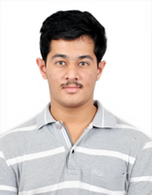
\includegraphics[width=2.5cm, height=2.6cm]{SohamBhave.jpg} \\
\end{tabular}

\section{\sc Objective}

Seeking an internship at a reputed organization which provides an opportunity to enhance my skills and challenge my abilities.

\section{\sc Education}
\begin{tabular}{ |c|c|c|c|c| } 
 \hline
 Degree & College & University & Passing Year & Pass Percentage \\ 
\hline 
B.E  E\&TC & MMCOE,Pune & SPPU & 2020 & 8.39(TE Sem-1) \\  
 \hline
\end{tabular}

\section{\sc Projects}
\begin{enumerate}
	\item Robocon 2018\\
	\begin{itemize}
		\item Worked with college’s Robocon team to design and manufacture robots.
		\item Primarily involved in path planning and odometry for an autonomous robot.
		\item Worked with a variety of sensors(Ultrasonic, IMU, Infrared, Rotary Encoders) and\\ actuators(DC 							Motors,linear pneumatic actuators)
		\item Programmed Microcontrollers (Atmega 16,Atmega 128,LPC 2148 ,Arduino) in\\ Embedded C	
	\end{itemize}
	\item Wrist mounted health monitor
	\begin{itemize}
		\item Built a wrist mounted system which could measure heart rate, body temperature and detect a person fallling over.
		\item It communicates this information over the internet via Blynk server to the concerned.  
		\item Worked with NodeMCU, Optical heart rate sensor, temperature sensor, OLED display
		\item Designed a PCB for the system
	\end{itemize}	
	\item Home Automation system to save Electricity
	\begin{itemize}
		\item Designed and developed a system which detected and counted the number of people in a room using 						ultrasonic sensors and the presence of light using an LDR.	
		\item Replaced the ordinary two way switches by relays.
		\item Using the data switched the tubelight and the fan by using an Arduino microcontroller	
	\end{itemize}
	\item Robotics Specialization on Coursera
	\begin{itemize}
		\item Implemented various simulation projects while completing courses under a Robotics specialization on Coursera. 				\item Specialization included courses on – Aerial Robotics, Robotic Motion Planning, Robotic Perception and Robotic 					Mobility by the University of Pennsylvania.	
		\item Simulations include :
		\begin{itemize}
			\item[--] 3D control(using PID) and trajectory planning of a quadrotor
			\item[--] Path planning algorithms 
			\item[--] 3D projection and pose estimation from visual data.
		\end{itemize}
	\end{itemize}
\end{enumerate}

\section{\sc Training and Internships}
\begin{itemize}
\item Intern at Grind Master Machines, Aurangabad (15th December 2018 – 17th January 2019)
\begin{itemize}
	\item Developed a machine learning algorithm to determine the touch time for superfinishing/ micro-finishing processes based 				on the input roughness parameters of the job to achieve desired target roughness parameters.
	\item Collected the data for implementing machine learning algorithm by processing jobs and then measuring their roughness 				parameters
	\item Implemented linear regression on the data to predict the expected touch time using Excel Macros.
	\item Evaluated the performance of the model on actual jobs for different processes.
\end{itemize}
\end{itemize}

\section{\sc Research Publication}
\begin{itemize}
	\item None
\end{itemize}

\section{\sc Technical Skills}
\begin{itemize}
	\item Programming languages : 
	\begin{itemize}
		\item C, C++
		\item Python, Java
	\end{itemize}
	\item Operating systems : 
	\begin{itemize}
		\item Windows
		\item Linux
	\end{itemize}
	\item Softwares :
	\begin{itemize}
		 \item MS Office, Matlab
		\item Circuit Design : Proteus, Multisim
	\end{itemize}
	\item Circuit designing, PCB designing, Soldering
\end{itemize}

\section{\sc Soft Skills}
\begin{enumerate}
	\item Verbal and non-verbal communication
	\item Teamwork
	\item Problem-solving skills
	\item Work Ethic
\end{enumerate}

\section{\sc Extra Curricular Activities}
\begin{itemize}
	\item Sports like football, cricket and badminton
\end{itemize}

\section{\sc Co-Curricular Activities}
\begin{enumerate}
	\item Participant in Robocon 2018 
	\item Participant in E-YRC 2017
\end{enumerate}

\section{\sc Personal Details}
\begin{itemize}
	\item Father's Name: Nikhil.M.Bhave
	\item Mother's Name: Suvarna.N.Bhave
	\item Sex: Male
	\item Date of Birth: 17-02-1998
	\item Nationality: Indian
	\item Marital Status: Single
\end{itemize}

\section{\sc Reference}
Available on request

\section{\sc Declaration}
I hereby declare that all the above mentioned information given by me is true and correct to the best of my knowledge and belief. \\\
\\
Place : Pune     
\hspace{10cm}       
Soham.N.Bhave

\end{resume}
\end{document}




